\section[碱金属光谱的精细结构]{碱金属光谱的精细结构} \label{sec:07.03} % 
% \makebox[5em][s]{} % 短题目拉间距

碱金属的原子价为1.价电子(最外层的一个电子)在原子核及内层电子的综合库仑场作用下运动,作用势可以近似地用一个中心势$V(r)$表示,这是决定价电子能级的主要物理因素.而能级与光谱的精细结构则来自更微弱的相对论性的物理因素,其中主要的一项称为自旋轨道耦合能,表现形式是
\begin{empheq}{equation}\label{eq73.1}
	\hat{H}^{\prime}=\xi(r)\boldsymbol{S}\cdot\boldsymbol{L}
\end{empheq}
$\boldsymbol{S},\boldsymbol{L}$是价电子的自旋及轨道角动量算符,$\xi(r)$是径向函数,按照相对论性的狄拉克方程,$\xi(r)$的函数形式是
\begin{empheq}{equation}\label{eq73.2}
	\xi(r)=\frac{1}{2m_{e}^{2}c^{2}}\frac{1}{r}\frac{dV}{dr}
\end{empheq}
对于类氢原子,
\begin{empheq}{equation}\label{eq73.3}
	V(r)=-\frac{Z\e^{2}}{r},\quad \xi(r)=\frac{Z\e^{2}}{2m_{e}^{2}c^{2}}\frac{1}{r^{3}}
\end{empheq}
例如氢原子$(Z=1)$,自旋轨道耦合能为
\begin{empheq}{equation}\label{eq73.4}
	\hat{H}^{\prime}=\frac{\e^{2}}{2m_{e}c^{2}}\frac{1}{r^{3}}\boldsymbol{S}\cdot\boldsymbol{L}
\end{empheq}
对于\eqref{eq73.4}式,常给予下述形式上的解释:电子在中心力场$V(r)$作用下形成的“轨道”运动(波函数$\varPsi_{nlm}$)造成空间电流,产生磁场,其电磁学效果可以用位于力心处$(r=0)$的“轨道磁矩”
\begin{empheq}{equation}\label{eq73.5}
	\boldsymbol{\mu}_{L}=-\frac{\e}{2m_{e}c}\boldsymbol{L}
\end{empheq}
来代替.电子又有自旋磁矩
\begin{empheq}{equation}\label{eq73.6}
	\boldsymbol{\mu}_{s}=-\frac{\e}{m_{e}c}\boldsymbol{S}
\end{empheq}
这两个磁矩(相距$\boldsymbol{r}$)之间的作用势为
\begin{empheq}{equation*}
	H^{\prime}=\frac{\boldsymbol{\mu}_{s}\cdot\boldsymbol{\mu}_{L}}{r^{3}}-\frac{3}{r^{5}}(\boldsymbol{\mu}_{s}\cdot\boldsymbol{r})(\boldsymbol{\mu}_{L}\cdot\boldsymbol{r})
\end{empheq}
由于$\boldsymbol{L}=\boldsymbol{r}\times\boldsymbol{p}=-\boldsymbol{p}\times\boldsymbol{r}$,所以$\boldsymbol{L}\cdot\boldsymbol{r}=0$,因此$\mu_{L}\cdot\boldsymbol{r}$,上式就变成\eqref{eq73.4}式.当然,这只能当作一种通俗的解释.

\eqref{eq73.4}式中,$\boldsymbol{S},\boldsymbol{L}$的量级为$\hbar$,$r$的量级为玻尔半径$a_{0}$,因此
\eqlong
\begin{empheq}{equation*}
	H^{\prime}\sim\frac{\e^{2}\hbar^{2}}{m_{e}^{2}c^{2}a_{0}^{3}}\sim\frac{\e^{2}}{a_{0}}\bigg(\frac{\e^{2}}{\hbar c}\bigg)^{2}\sim\frac{27\si{eV}}{(137)^{2}}\sim\num{1.4}\times 10^{-3}\si{eV}
\end{empheq}\eqnormal
按量级说,自旋轨道耦合能$H^{\prime}$约为电子能级的$10^{-4}\sim10^{-3}$倍,所以可以作为微扰处理.价电子的总能量算符表示成
\begin{empheq}{equation}\label{eq73.7}
	H=H_{0}+H^{\prime},\quad H_{0}=\frac{\boldsymbol{p}^{2}}{2m_{e}}+V(r)
\end{empheq}
与$H$对易的力学量(守恒量)有$H,\boldsymbol{L}^{2},\boldsymbol{J}^{2},J_{x},J_{y},J_{z}$.注意,不考虑自旋轨道耦合作用时(取$H\sim H_{0}$),$\boldsymbol{L},\boldsymbol{S}$都是守恒量.由于$H^{\prime}$的存在,$\boldsymbol{L},\boldsymbol{S}$已经不是守恒量,守恒的是能量,总角动量$\boldsymbol{J}=\boldsymbol{L}+\boldsymbol{S}$,以及$\boldsymbol{L}^{2}$.

守恒量完全集可以取为$(H,\boldsymbol{L}^{2},\boldsymbol{J}^{2},J_{z})$,它们的共同本征函数记为$\Psi_{nljm_{j}}(r,\theta,\varphi,S_{z})$,相应于本征值$H=E_{nlj}$以及
\eqlong
\begin{empheq}{equation}\label{eq73.8}
	\boldsymbol{L}^{2}=l(l+1)\hbar^{2},\quad \boldsymbol{J}^{2}=j(j+1)\hbar^{2},\quad J_{z}=m_{j}\hbar
\end{empheq}\eqnormal
一般的中心力场,能级记为$E_{nl}$,现在由于存在自旋轨道耦合能,能级也与之值有关,亦即与$j$有关.但$\boldsymbol{S}\cdot\boldsymbol{L}$之值与$m_{j}$无关,所以能级也与$m_{j}$无关.能级$E_{nlj}$的简并度为$(2j+1)$,相应于$(2j+1)$种$m_{j}$的取值
\begin{empheq}{equation}\label{eq73.9}
	m_{j}=j,j-1,\cdots,(-j)
\end{empheq}
能级的计算可以用微扰论.由于$H_{0}$与$\boldsymbol{L},\boldsymbol{J}$均可对易,可以取$(H_{0},\boldsymbol{L}^{2},\boldsymbol{J}^{2},J_{z})$的共同本征函数作为微扰论的零级近似波函数,记为
\begin{empheq}{equation}\label{eq73.10}
	\Psi_{nljm_{j}}^{(0)}=R_{nl}^{(0)}(r)\varPsi_{ljm_{j}}(\theta,\varphi,S_{z})
\end{empheq}
$\varPsi_{ljm_{j}}$就是$\S$\ref{sec:07.02}讨论过的$(\boldsymbol{L}^{2},\boldsymbol{J}^{2},J_{z})$共同本征函数.$R_{nl}^{(0)}$是径向波函数,与能级的零级近似(记为$E_{nl}^{(0)}$)一起由径向方程(势能$V$)解出.由于微扰$H^{\prime}$与$(\boldsymbol{L}^{2},\boldsymbol{J}^{2},J_{z})$均对易,按照简并态微扰论,\eqref{eq73.10}式就是正确的零级波函数,能级的一级修正等于$H^{\prime}$的平均值,即
\eqlong
\begin{empheq}{align}\label{eq73.11}
	E_{nlj}^{(1)}&=\langle H^{\prime}\rangle=\int\Psi_{nljm_{j}}^{(0)+}\xi(r)\boldsymbol{S}\cdot\boldsymbol{L}\Psi_{nljm_{j}}^{(0)}d\tau	\nonumber\\
	&=\langle\xi(r)\rangle(\boldsymbol{S}\cdot\boldsymbol{L}\text{本征值})
\end{empheq}
其中
\begin{empheq}{equation}\label{eq73.12}
	\langle\xi(r)\rangle=\int_{0}^{\infty}\xi(r)[R_{nl}^{(0)}(r)]^{2}r^{2}dr>0
\end{empheq}
\begin{empheq}{equation}\label{eq73.13}
	{\boldsymbol{S}\cdot\boldsymbol{L}\text{本征值}=}
	\begin{dcases}
		\quad \frac{l\hbar^{2}}{2},\qquad j=l+\frac{1}{2}	\\
		-\frac{(l+1)\hbar^{2}}{2},\quad j=l-\frac{1}{2}
	\end{dcases}
\end{empheq}\eqnormal
准确到一级近似,能级($H$的本征值)可以表示成
\begin{empheq}{equation}\label{eq73.14}
	E_{nlj}\approx E_{nl}^{(0)}+E_{nlj}^{(0)}
\end{empheq}
\begin{wrapfigure}[8]{r}{7em}
	\centering
	\small
	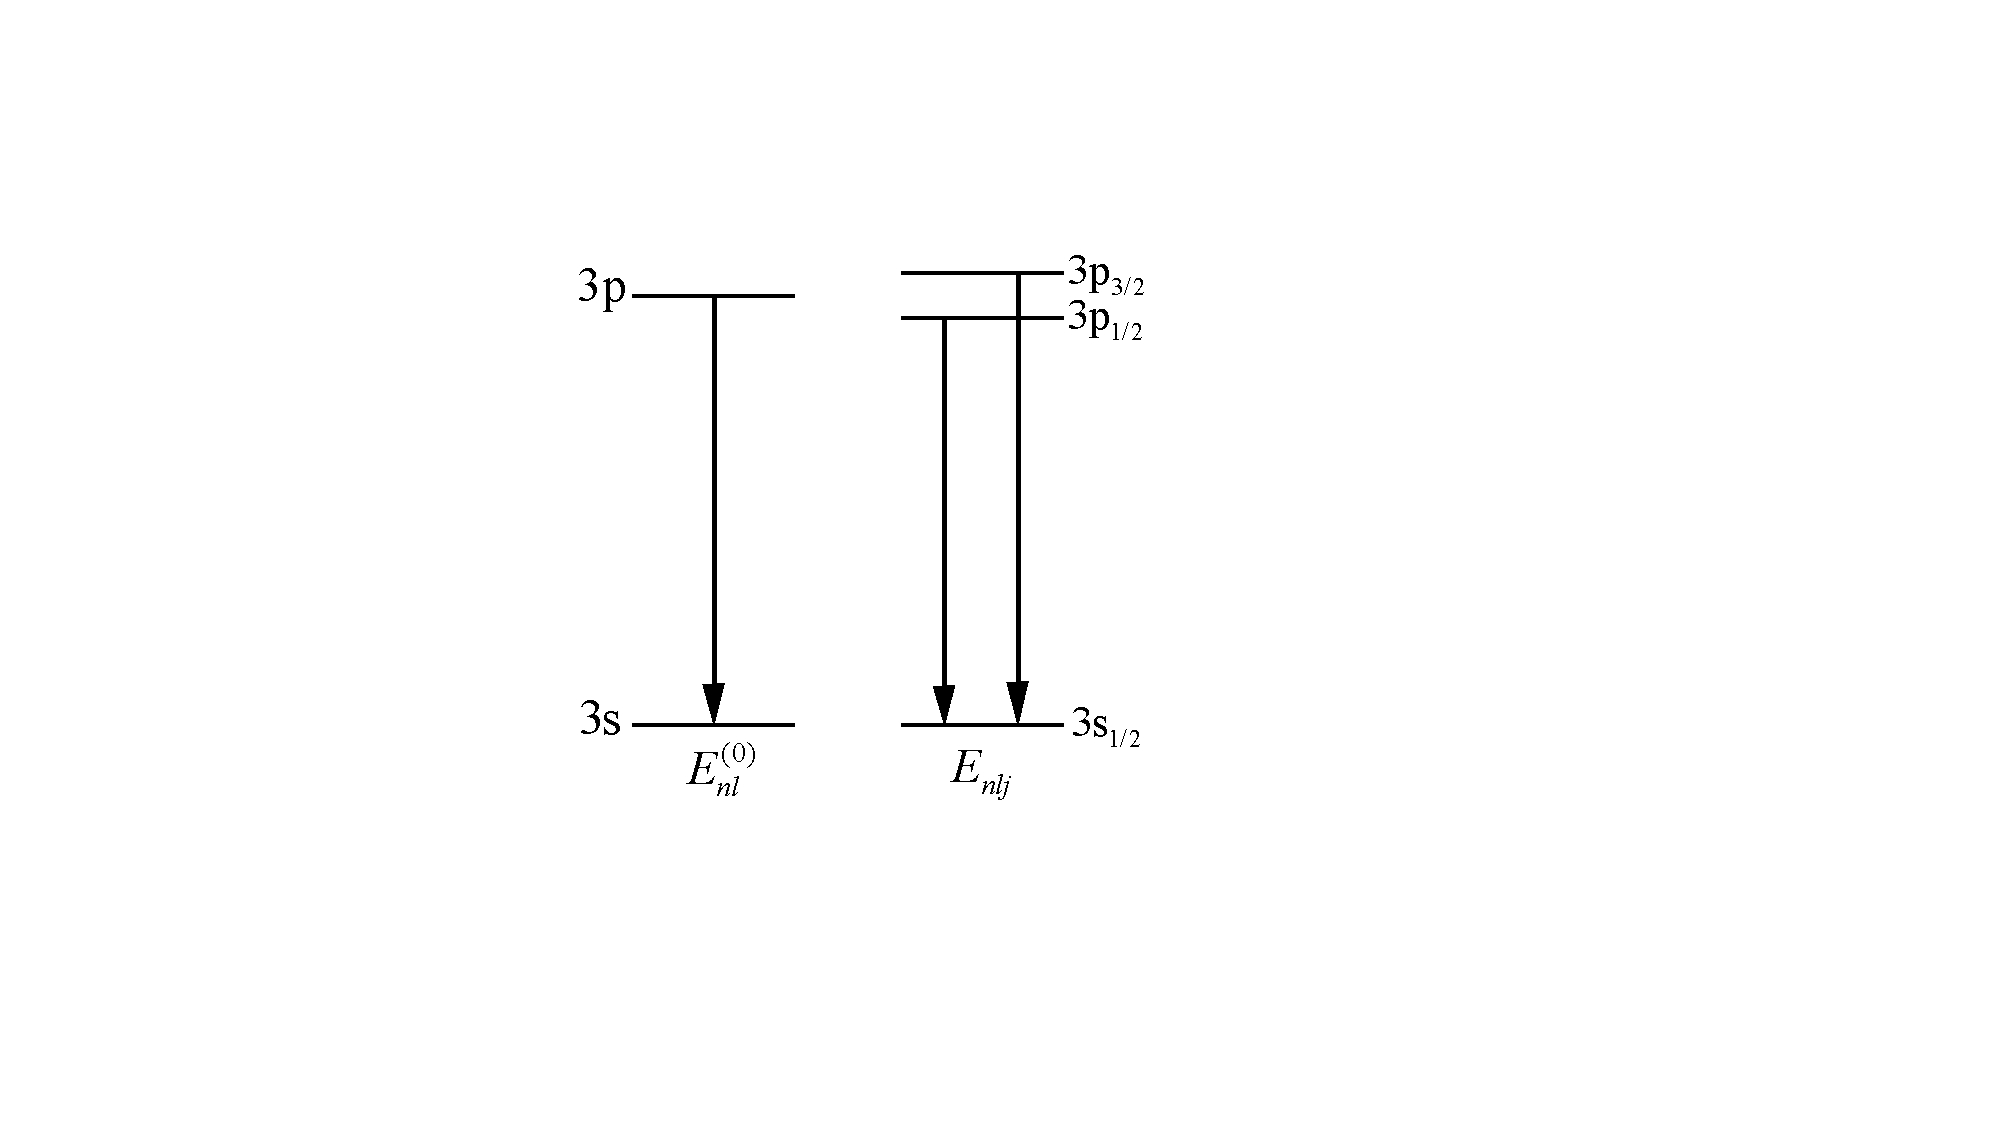
\includegraphics[width=3cm,clip]{QM file/figure/7-1}
	\caption{}\label{fig.7-1}
\end{wrapfigure}
由于自旋轨道耦合作用,能级$E_{nl}^{(0)}$分裂成两个能级,$j=l+\frac{1}{2}$者较高$(E_{nlj}^{(1)}>0)$,$j=l-\frac{1}{2}$者较低$(E_{nlj}^{(1)}<0)$,裂距
\eqllong
\begin{empheq}{align}\label{eq73.15}
	\Delta E&=E_{nl,l+\frac{1}{2}}^{(1)}-E_{nl,l-\frac{1}{2}}^{(1)}	\nonumber\\
	&=\bigg(l+\frac{1}{2}\bigg)\hbar^{2}\langle\xi(r)\rangle 
\end{empheq}\eqnormal
但s态例外,s态$\boldsymbol{S}\cdot\boldsymbol{L}\text{(本征值)}=0$,没有自旋轨道耦合能,能级不分裂.

能级分裂的示意图见图\ref{fig.7-1},图中画出了3p$(n=3,l=1)$能级的分裂情况与此相应,跃迁3p$\rightarrow$3s造成的光谱线也分裂成两条,这就是光谱线的精细结构.








